\documentclass[11pt,a4paper]{article}
% ---------------------------------------------------------------------------
%  PHAROS technical paper -- shared preamble
% ---------------------------------------------------------------------------
\usepackage[utf8]{inputenc}
\usepackage[T1]{fontenc}
\usepackage{lmodern}
\usepackage[margin=2.3cm]{geometry}
\usepackage{amsmath,amssymb,amsthm}
\usepackage{booktabs}
\usepackage{multirow}
\usepackage{longtable}
\usepackage{array}
\usepackage{xcolor}
\usepackage{microtype}
\usepackage{caption}
\usepackage{subcaption}
\usepackage{enumitem}
\usepackage{fancyhdr}
\usepackage{float}
\usepackage{siunitx}
\usepackage[hidelinks,colorlinks=true,linkcolor=linknavy,citecolor=linknavy,
            urlcolor=linknavy]{hyperref}

\usepackage{tikz}
\usetikzlibrary{arrows.meta,positioning,calc,fit,backgrounds,shapes.geometric,
                decorations.pathreplacing,decorations.pathmorphing,patterns,
                shadows.blur,matrix,chains,shapes.misc}
\usepackage{pgfplots}
\pgfplotsset{compat=1.18}

% ---- palette -------------------------------------------------------------
\definecolor{linknavy}{HTML}{1F3A5F}
\definecolor{trunkblue}{HTML}{2C5282}
\definecolor{trunkbg}{HTML}{EBF2FA}
\definecolor{moeorange}{HTML}{B45309}
\definecolor{moebg}{HTML}{FEF3C7}
\definecolor{headgreen}{HTML}{276749}
\definecolor{headbg}{HTML}{E6F4EA}
\definecolor{diffpurple}{HTML}{553C9A}
\definecolor{diffbg}{HTML}{EDE9F7}
\definecolor{datagrey}{HTML}{4A5568}
\definecolor{databg}{HTML}{EDF2F7}
\definecolor{physteal}{HTML}{14687A}
\definecolor{physbg}{HTML}{E0F2F5}
\definecolor{newred}{HTML}{9B2C2C}
\definecolor{newbg}{HTML}{FDE8E8}
\definecolor{rule1}{HTML}{CBD5E0}

% ---- shared tikz styles --------------------------------------------------
\tikzset{
  blk/.style={rounded corners=2pt, draw=#1, line width=0.7pt, fill=#1!6,
              align=center, inner sep=4pt, font=\small},
  tag/.style={font=\scriptsize\itshape, text=datagrey},
  flow/.style={-{Stealth[length=2.4mm,width=1.8mm]}, line width=0.75pt,
               draw=datagrey},
  flowthick/.style={-{Stealth[length=3mm,width=2.4mm]}, line width=1.3pt,
                    draw=datagrey},
  dashflow/.style={-{Stealth[length=2.4mm,width=1.8mm]}, line width=0.7pt,
                   draw=datagrey, dashed, dash pattern=on 2.4pt off 1.8pt},
  lbl/.style={font=\scriptsize, inner sep=1.5pt, fill=white, text=datagrey},
  note/.style={font=\scriptsize, text=datagrey, align=left},
}

% ---- semantic macros -----------------------------------------------------
\newcommand{\pharos}{\textsc{Pharos}}
\newcommand{\fnd}[1]{\textcolor{newred}{\footnotesize\,[F#1]}}
\newcommand{\code}[1]{\texttt{\small #1}}
\newcommand{\angs}{\si{\angstrom}}
\newcommand{\Ang}{\text{\AA}}
\DeclareMathOperator{\RBF}{RBF}
\DeclareMathOperator{\softmax}{softmax}
\DeclareMathOperator{\cdist}{cdist}

\captionsetup{font=small,labelfont=bf,width=0.95\textwidth}
\setlist{itemsep=1pt,topsep=3pt,parsep=0pt}

\pagestyle{fancy}
\fancyhf{}
\lhead{\small\textsc{Pharos}: architecture as built}
\rhead{\small\thepage}
\renewcommand{\headrulewidth}{0.4pt}


\title{\textbf{\textsc{Pharos}}\\[0.35em]
\large A physics-grounded mixture-of-experts architecture\\
for RNA three-dimensional structure prediction\\[0.7em]
\normalsize Technical report --- the architecture as built, and what it measures}
\author{SBS-RNA Project}
\date{10 October 2026}

\begin{document}
\maketitle

\begin{abstract}
\noindent
This report documents \pharos{} as it exists in code, not as it was
designed. It is a 395.3M-parameter model (306.0M active) that predicts RNA
secondary structure, chemical reactivity, contacts, distances,
Leontis--Westhof pair geometry, Mg$^{2+}$ sites, crystallographic
rigidity, backbone pseudotorsions and three-dimensional backbone
coordinates, trained through a six-stage curriculum from a 41.2M-sequence
masked-language-modelling corpus down to a 16{,}604-chain
structural set.

We report what it achieves, which is a mean TM-score of
$\mathbf{0.094}$ over 17 RNA-Puzzles targets against a field median of
$0.301$ --- last place on 15 of 17 --- alongside a contact average
precision of $0.890$ and an lDDT of $0.269$. That combination is the
central empirical fact of this report: \textbf{the model builds
locally-valid RNA backbone and places it in the wrong global
arrangement}. We trace it to a specific architectural omission, give the
fix, and are explicit that the fix is not yet measured.

The second contribution is methodological. The project maintains a
numbered defect register, at present 104 entries, whose recurring class
is \emph{a component that exists, is measured, and whose output is never
checked for basic validity}. Several entries are errors in our own
instrumentation rather than in the model, and are recorded as such.
We argue this bookkeeping is not incidental to the work but is the main
reason the negative results above can be trusted.
\end{abstract}

\tableofcontents
\bigskip

% =========================================================================
\section{What problem this is}

RNA structure prediction has not had its AlphaFold2 moment. On
non-redundant benchmarks the best current methods reach mean TM-scores
around $0.5$--$0.6$, where $0.45$ is roughly the threshold for having
recovered the correct fold at all, against routine scores above $0.9$ for
proteins. The usual explanations are that there are two orders of
magnitude fewer RNA structures than protein structures, that RNA's
functional unit is often a conformational ensemble rather than one
structure, and that RNA folding is ion-dependent in a way protein folding
is not.

\pharos{} takes a position on which of these matters: that the binding
constraint is \emph{inductive bias} rather than scale, and that the
physics of ion condensation and the geometry of base pairing should enter
the architecture rather than be left for the network to rediscover. This
report does not defend that position --- it was argued in the design
report that preceded the implementation --- but documents what was built
from it and what that produced.

\paragraph{A note on what this report is not.} It reports a model that
does not work yet at the task it was built for. The results section is
written to be useful to that end rather than flattering, and every number
in it is traceable to a file in the repository.

% =========================================================================
\section{Architecture}

\begin{figure}[H]\centering
\resizebox{\textwidth}{!}{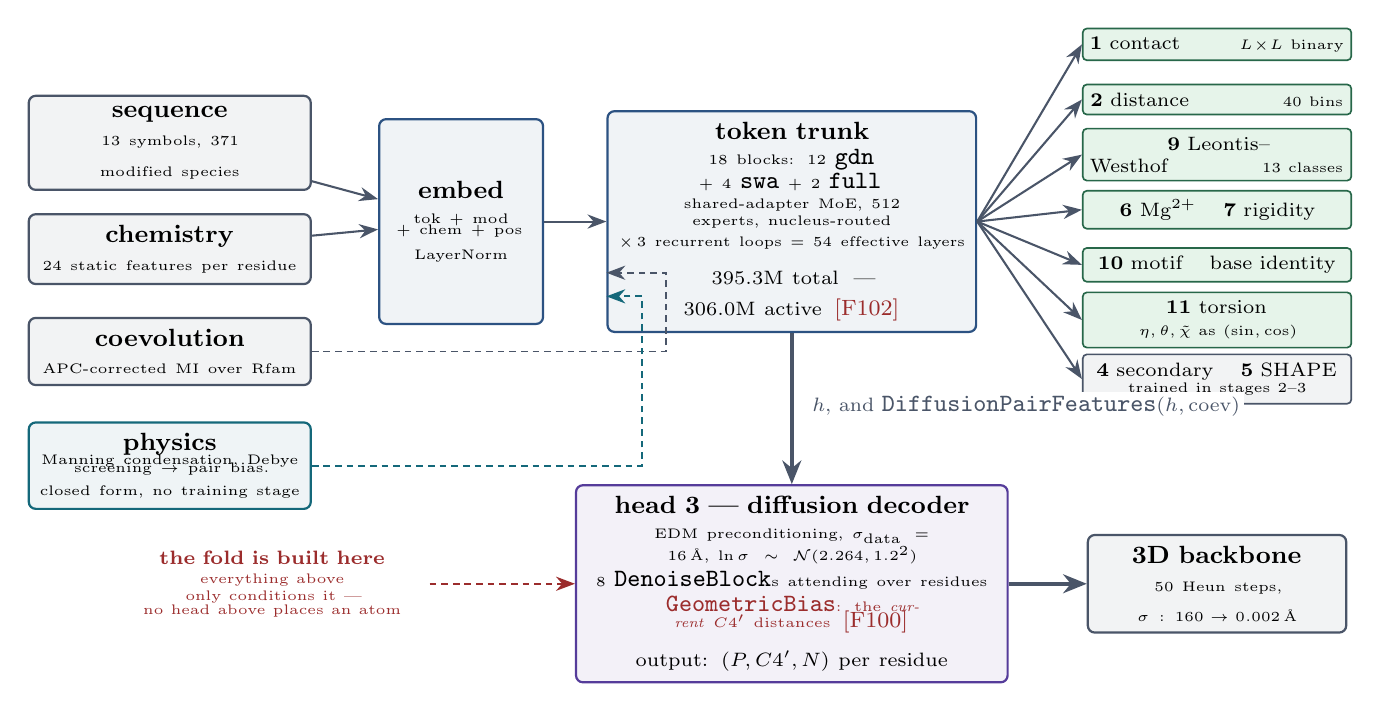
\begin{tikzpicture}[font=\small]
\tikzset{
  st/.style={rounded corners=2.5pt, draw=#1, line width=0.8pt, fill=#1!7,
             align=center, inner sep=4pt, font=\small},
  hd/.style={rounded corners=1.5pt, draw=headgreen, line width=0.6pt,
             fill=headbg, align=center, inner sep=3pt, font=\scriptsize,
             text width=32mm},
}

% ------------------------- inputs ---------------------------------------
\node[st=datagrey, text width=33mm] at (0, 0.05) (seq)
   {\textbf{sequence}\\[-1pt]\tiny 13 symbols, 371 modified species};
\node[st=datagrey, text width=33mm] at (0,-1.30) (chem)
   {\textbf{chemistry}\\[-1pt]\tiny 24 static features per residue};
\node[st=datagrey, text width=33mm] at (0,-2.60) (msa)
   {\textbf{coevolution}\\[-1pt]\tiny APC-corrected MI over Rfam};
\node[st=physteal, text width=33mm] at (0,-4.05) (phys)
   {\textbf{physics}\\[-1pt]\tiny Manning condensation, Debye\\[-3pt]
    \tiny screening $\to$ pair bias.\\[-3pt]\tiny closed form, no training stage};

\node[st=trunkblue, text width=18mm, minimum height=26mm] at (3.7,-0.95) (emb)
   {\textbf{embed}\\[3pt]\tiny tok $+$ mod\\[-2pt]\tiny $+$ chem $+$ pos\\[-2pt]
    \tiny LayerNorm};
\draw[flow] (seq)  -- (emb); \draw[flow] (chem) -- (emb);

% ------------------------- trunk ----------------------------------------
\node[st=trunkblue, text width=44mm, minimum height=26mm] at (7.9,-0.95) (trunk)
   {\textbf{token trunk}\\[3pt]
    \tiny 18 blocks: 12 \code{gdn} $+$ 4 \code{swa} $+$ 2 \code{full}\\[1.5pt]
    \tiny shared-adapter MoE, 512 experts, nucleus-routed\\[1.5pt]
    \tiny $\times\,3$ recurrent loops $=$ 54 effective layers\\[3pt]
    \scriptsize $395.3$M total \;|\; $306.0$M active \fnd{102}};
\draw[flow] (emb) -- (trunk);
\draw[dashflow, draw=datagrey]  (msa.east)  -| (6.3,-1.6) -- (trunk.west|-0,-1.6);
\draw[dashflow, draw=physteal]  (phys.east) -| (6.0,-1.9) -- (trunk.west|-0,-1.9);

% ------------------------- heads ----------------------------------------
\node[hd] at (13.3, 1.30) (h1) {\textbf{1} contact\hfill\tiny $L\!\times\!L$ binary};
\node[hd] at (13.3, 0.60) (h2) {\textbf{2} distance\hfill\tiny 40 bins};
\node[hd] at (13.3,-0.10) (h9) {\textbf{9} Leontis--Westhof\hfill\tiny 13 classes};
\node[hd] at (13.3,-0.80) (h6) {\textbf{6} Mg$^{2+}$ \;\; \textbf{7} rigidity};
\node[hd] at (13.3,-1.50) (h10){\textbf{10} motif \;\; base identity};
\node[hd] at (13.3,-2.20) (h11){\textbf{11} torsion\hfill\tiny $\eta,\theta,\tilde\chi$ as $(\sin,\cos)$};
\node[hd, draw=datagrey, fill=datagrey!7] at (13.3,-2.95) (hu)
   {\textbf{4} secondary \;\; \textbf{5} SHAPE\\[-2pt]\tiny trained in stages 2--3};
\foreach \n in {h1,h2,h9,h6,h10,h11,hu}{\draw[flow] (trunk.east) -- (\n.west);}

% ------------------------- decoder --------------------------------------
\node[st=diffpurple, text width=52mm, minimum height=21mm] at (7.9,-5.55) (dec)
   {\textbf{head 3 --- diffusion decoder}\\[3pt]
    \tiny EDM preconditioning, $\sigma_{\text{data}}=16\,\Ang$,
      $\ln\sigma\sim\mathcal{N}(2.264,1.2^2)$\\[1.5pt]
    \tiny 8 \code{DenoiseBlock}s attending over residues\\[1.5pt]
    \tiny\textcolor{newred}{\code{GeometricBias}: the \emph{current} $C4'$
      distances} \fnd{100}\\[3pt]
    \scriptsize output: $(P, C4', N)$ per residue};
\draw[flowthick] (trunk.south) -- (dec.north);
\node[lbl, anchor=west] at (8.1,-3.3)
   {\scriptsize $h$, and \code{DiffusionPairFeatures}$(h,\text{coev})$};

\node[st=datagrey, text width=30mm] at (13.3,-5.55) (out)
   {\textbf{3D backbone}\\[-1pt]\tiny 50 Heun steps,
    $\sigma:160\!\to\!0.002\,\Ang$};
\draw[flowthick] (dec) -- (out);

\node[note, align=center, text width=36mm, text=newred] at (1.3,-5.55)
   {\textbf{the fold is built here}\\[1pt]
    \tiny everything above only conditions it ---\\[-3pt]
    \tiny no head above places an atom};
\draw[dashflow, draw=newred] (3.3,-5.55) -- (dec.west);
\end{tikzpicture}
}
\caption{\textbf{\pharos{} end to end.} A shared trunk produces one
residue representation $h$ that every head reads. Ten heads are trained
discriminative readouts; the eleventh, head~3, is a diffusion decoder
that is the only component that places an atom. The physics module
contributes a closed-form electrostatic pair bias and has no training
stage of its own. Bracketed numbers are defect-register entries
discussed in \S\ref{sec:register}.}
\label{fig:system}
\end{figure}

\subsection{Inputs}

Each residue carries four things, summed and layer-normalised:

\begin{itemize}
\item a \textbf{symbol} from a 13-token vocabulary
  (\texttt{A C G U N DA DC DG DT DU I UNK PAD}), where \texttt{N} means
  the ribose is modelled but the base identity is unassigned;
\item a \textbf{modification} id over 371 species (index 0 is
  \texttt{NO\_MOD}), derived from the chemical component dictionary, so
  that a pseudouridine is not silently read as a uridine;
\item 24 \textbf{chemistry} features through a single affine map ---
  a 5-way one-hot, a purine flag, six per-edge hydrogen-bond
  donor/acceptor counts (Watson--Crick, Hoogsteen/CH, sugar), the p$K_a$
  of the protonating ring nitrogen and a shifted-p$K_a$ flag, two sugar
  pucker propensities, polarisability and a stacking-energy prior, the
  phosphate charge state, a 2$'$-OH flag, three modification-class
  indicators, and local GC fraction in a $\pm16$ window;
\item a \textbf{learned absolute position} embedding over 4{,}608 slots.
  There is no rotary or sinusoidal encoding anywhere in the model.
\end{itemize}

\subsection{The trunk}

\begin{figure}[H]\centering
\resizebox{\textwidth}{!}{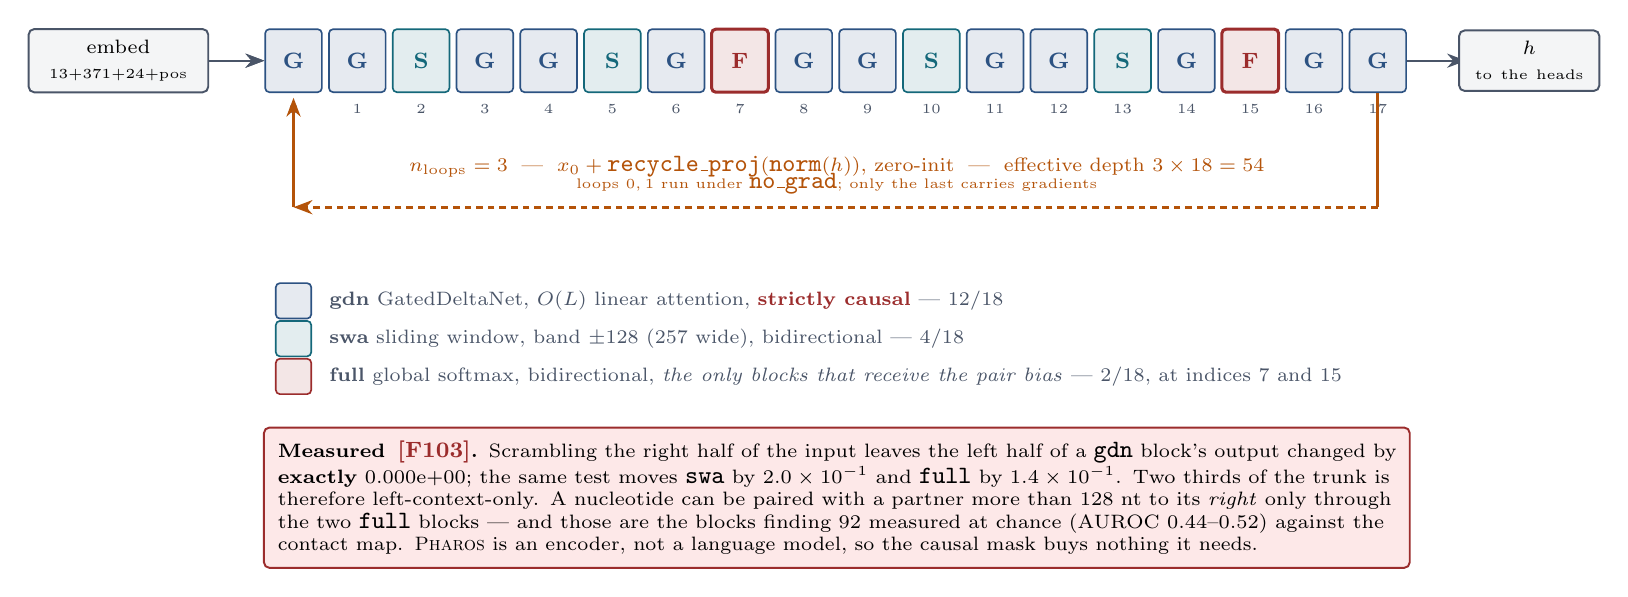
\begin{tikzpicture}[font=\small]
\tikzset{
  bk/.style={rounded corners=1.5pt, draw=#1, line width=0.6pt, fill=#1!12,
             minimum width=7.2mm, minimum height=8mm, inner sep=0pt,
             font=\footnotesize\bfseries, text=#1},
  leg/.style={rounded corners=1.5pt, draw=#1, line width=0.6pt, fill=#1!12,
              minimum width=4.5mm, minimum height=4.5mm, inner sep=0pt},
}
% block kinds, written out: the period-8 pattern tiled to 18
% G G S G G S G F | G G S G G S G F | G G
\foreach \i in {0,1,3,4,6,8,9,11,12,14,16,17}{
  \node[bk=trunkblue] at (\i*8.1mm,0) (b\i) {G};}
\foreach \i in {2,5,10,13}{
  \node[bk=physteal] at (\i*8.1mm,0) (b\i) {S};}
\foreach \i in {7,15}{
  \node[bk=newred, line width=1.1pt] at (\i*8.1mm,0) (b\i) {F};}
\foreach \i in {0,...,17}{
  \node[font=\tiny, text=datagrey] at (\i*8.1mm,-0.62) {\i};}

\draw[flow] (-0.72,0) -- (b0.west);
\node[blk=datagrey, left=1mm of b0, xshift=-6mm, text width=20mm, align=center]
   (emb) {\scriptsize embed\\[-2pt]\tiny $13{+}371{+}24{+}\mathrm{pos}$};
\draw[flow] (emb) -- (b0);
\draw[flow] (b17.east) -- ++(0.75,0) node[right, blk=datagrey, text width=15mm,
   align=center, anchor=west, xshift=-1mm] (hid) {\scriptsize $h$\\[-2pt]\tiny to the heads};

% ---------- the recurrence ----------------------------------------------
\draw[dashflow, draw=moeorange, line width=1pt]
   ($(b17.south)+(0,-1.45)$) -- ($(b0.south)+(0,-1.45)$);
\draw[draw=moeorange, line width=1pt] (b17.south) -- ($(b17.south)+(0,-1.45)$);
\draw[-{Stealth[length=2.4mm]}, draw=moeorange, line width=1pt]
   ($(b0.south)+(0,-1.45)$) -- ($(b0.south)+(0,-0.06)$);
\node[font=\scriptsize, text=moeorange, align=center, fill=white, inner sep=1.5pt]
   at (6.9,-1.45) {$n_{\text{loops}}=3$ \;|\; $x_0 + \code{recycle\_proj}(\code{norm}(h))$,
     zero-init \;|\; effective depth $3\times18=54$\\[-2pt]
     \tiny loops $0,1$ run under \code{no\_grad}; only the last carries gradients};

% ---------- legend -------------------------------------------------------
\begin{scope}[shift={(0,-3.05)}]
  \node[leg=trunkblue] at (0,0) {}; \node[note, anchor=west] at (0.33,0)
    {\textbf{gdn} GatedDeltaNet, $O(L)$ linear attention, \textbf{\textcolor{newred}{strictly causal}} --- $12/18$};
  \node[leg=physteal] at (0,-0.48) {}; \node[note, anchor=west] at (0.33,-0.48)
    {\textbf{swa} sliding window, band $\pm128$ (257 wide), bidirectional --- $4/18$};
  \node[leg=newred] at (0,-0.96) {}; \node[note, anchor=west] at (0.33,-0.96)
    {\textbf{full} global softmax, bidirectional, \emph{the only blocks that receive the pair bias} --- $2/18$, at indices $7$ and $15$};
\end{scope}

% ---------- the causality note ------------------------------------------
\node[draw=newred, fill=newbg, rounded corners=2pt, line width=0.7pt,
      text width=142mm, align=left, font=\scriptsize, inner sep=5pt]
   at (6.9,-5.55)
   {\textbf{Measured \fnd{103}.} Scrambling the right half of the input leaves
    the left half of a \code{gdn} block's output changed by \textbf{exactly
    $0.000\mathrm{e}{+}00$}; the same test moves \code{swa} by
    $2.0\times10^{-1}$ and \code{full} by $1.4\times10^{-1}$. Two thirds of
    the trunk is therefore left-context-only. A nucleotide can be paired with
    a partner more than $128$~nt to its \emph{right} only through the two
    \code{full} blocks --- and those are the blocks finding~92 measured at
    chance (AUROC $0.44$--$0.52$) against the contact map. \pharos{} is an
    encoder, not a language model, so the causal mask buys nothing it needs.};
\end{tikzpicture}
}
\caption{\textbf{The 18-block trunk.} A period-8 attention pattern tiled
to 18 blocks, run three times with the previous pass recycled in. The
annotation records a property we measured rather than assumed, and which
we regard as an open question rather than a settled defect.}
\label{fig:trunk}
\end{figure}

The trunk is 18 pre-norm blocks following the period-8 pattern
\texttt{(gdn, gdn, swa, gdn, gdn, swa, gdn, full)}, which tiles to twelve
\texttt{gdn}, four \texttt{swa} and two \texttt{full} at indices 7
and 15. Only the \texttt{full} blocks receive the electrostatic pair
bias, through a per-head gate initialised to zero.

\paragraph{\texttt{gdn} --- gated delta networks.} Linear attention with a
delta rule, $O(L)$ in sequence length. Per head, with state
$S \in \mathbb{R}^{d_k \times d_v}$,
\begin{equation}
S_t = a_t\,S_{t-1}\!\left(I - b_t k_t k_t^{\!\top}\right) + b_t v_t k_t^{\!\top},
\qquad o_t = S_t^{\!\top} q_t ,
\end{equation}
with $a_t,b_t \in (0,1)$ sigmoid gates, $q$ and $k$ $\ell_2$-normalised,
and an output gate on $o$. The delta term erases the component of the
state already associated with $k$ before writing, so a recurring motif
overwrites rather than accumulates --- on a helix, where the same local
geometry recurs every ${\sim}11$ nt, accumulation is precisely the
failure mode. It is evaluated chunkwise in blocks of 128 with a
triangular solve.

\paragraph{\texttt{swa} and \texttt{full}.} Sliding-window attention over
a band of $\pm128$ (257 wide), implemented densely with a band mask, and
ordinary global softmax attention.

\paragraph{Recurrence.} The entire trunk is run $n=3$ times with shared
weights, giving 54 effective layers. Loops $0$ and $1$ run under
\code{no\_grad} and only the last carries gradients, so the memory cost
is that of one pass. The recycled state enters as
$x_0 + \code{recycle\_proj}(\code{norm}(h))$ with \code{recycle\_proj}
initialised to zero, so loop 1 begins numerically identical to loop 0.
Training samples the depth uniformly from $1\ldots3$. There is no halting
mechanism.

\subsection{The mixture of experts}

\begin{figure}[H]\centering
\resizebox{0.98\textwidth}{!}{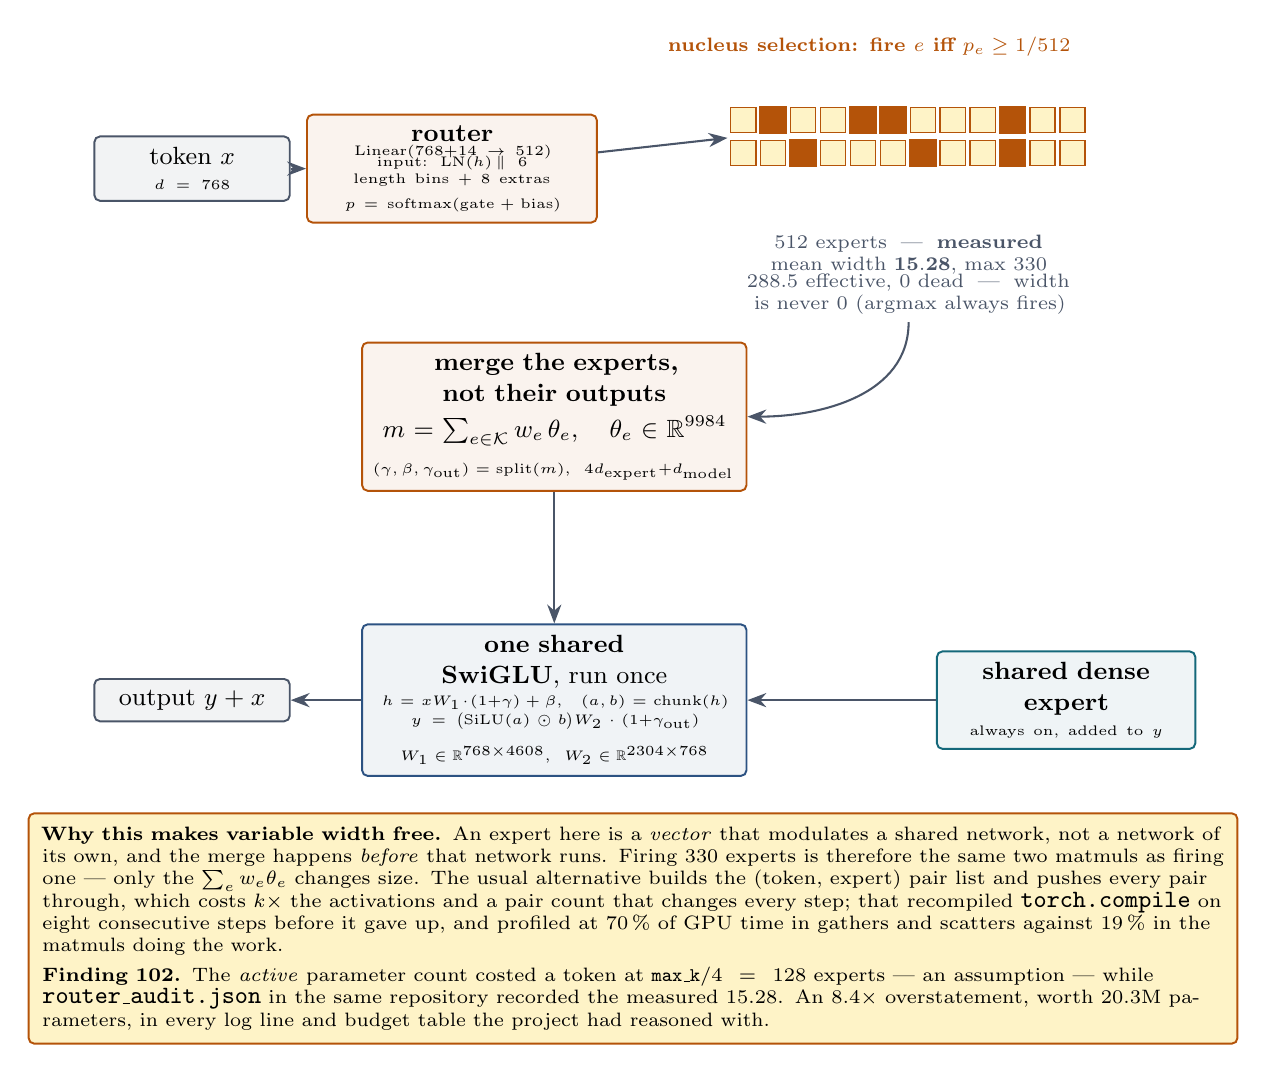
\begin{tikzpicture}[font=\small]
\tikzset{
  mb/.style={rounded corners=2pt, draw=#1, line width=0.7pt, fill=#1!7,
             align=center, inner sep=4pt, font=\small},
  ex/.style={draw=moeorange, line width=0.5pt, fill=moebg,
             minimum width=3.2mm, minimum height=3.2mm, inner sep=0pt},
  exon/.style={draw=moeorange, line width=0.9pt, fill=moeorange,
               minimum width=3.2mm, minimum height=3.2mm, inner sep=0pt},
}

% ---------------- token in -----------------------------------------------
\node[mb=datagrey, text width=22mm] at (0,0) (tok)
   {token $x$\\[-2pt]\tiny $d=768$};

% ---------------- router --------------------------------------------------
\node[mb=moeorange, text width=34mm] at (3.3,0) (gate)
   {\textbf{router}\\[-1pt]
    \tiny $\mathrm{Linear}(768{+}14 \to 512)$\\[-2pt]
    \tiny input: $\mathrm{LN}(h)\,\Vert\,$ 6 length bins $+$ 8 extras\\[-2pt]
    \tiny $p = \softmax(\text{gate} + \text{bias})$};
\draw[flow] (tok) -- (gate);

% ---------------- nucleus selection --------------------------------------
\node[font=\scriptsize\bfseries, text=moeorange] at (8.6,1.55)
  {nucleus selection: fire $e$ iff $p_e \ge 1/512$};
\foreach \i in {0,...,23}{
  \pgfmathsetmacro{\xx}{7.0 + mod(\i,12)*0.38}
  \pgfmathsetmacro{\yy}{0.62 - floor(\i/12)*0.42}
  \node[ex] at (\xx,\yy) {};
}
\foreach \i in {1,4,5,9,14,18,21}{
  \pgfmathsetmacro{\xx}{7.0 + mod(\i,12)*0.38}
  \pgfmathsetmacro{\yy}{0.62 - floor(\i/12)*0.42}
  \node[exon] at (\xx,\yy) {};
}
\node[note, align=center, text width=52mm] at (9.1,-1.35)
  {\scriptsize 512 experts \;|\; \textbf{measured} mean width
   $\mathbf{15.28}$, max 330\\[-2pt]
   \scriptsize 288.5 effective, 0 dead \;|\; width is never 0 (argmax always fires)};
\draw[flow] (gate) -- (6.80,0.39);

% ---------------- the merge ----------------------------------------------
\node[mb=moeorange, text width=46mm] at (4.6,-3.15) (merge)
   {\textbf{merge the experts, not their outputs}\\[2pt]
    $m = \sum_{e\in\mathcal{K}} w_e\,\theta_e$,
      \;\; $\theta_e \in \mathbb{R}^{9984}$\\[2pt]
    \tiny $(\gamma,\beta,\gamma_{\text{out}})
      = \mathrm{split}(m)$, \;$4d_{\text{expert}}{+}d_{\text{model}}$};
\draw[flow] (9.1,-1.95) to[out=270,in=0] (merge.east);

\node[mb=trunkblue, text width=46mm] at (4.6,-6.75) (swiglu)
   {\textbf{one shared SwiGLU}, run once\\[2pt]
    \tiny $h = xW_1\!\cdot\!(1{+}\gamma) + \beta$,\quad
      $(a,b)=\mathrm{chunk}(h)$\\[1pt]
    \tiny $y = \big(\mathrm{SiLU}(a)\odot b\big)W_2
      \cdot (1{+}\gamma_{\text{out}})$\\[2pt]
    \tiny $W_1\!\in\!\mathbb{R}^{768\times4608}$,\;
      $W_2\!\in\!\mathbb{R}^{2304\times768}$};
\draw[flow] (merge) -- (swiglu);

\node[mb=physteal, text width=30mm] at (11.1,-6.75) (shared)
   {\textbf{shared dense expert}\\[-2pt]\tiny always on, added to $y$};
\draw[flow] (shared) -- (swiglu);

\node[mb=datagrey, text width=22mm] at (0,-6.75) (out) {output $y + x$};
\draw[flow] (swiglu) -- (out);

% ---------------- the point ----------------------------------------------
\node[draw=moeorange, fill=moebg, rounded corners=2pt, line width=0.7pt,
      text width=150mm, align=left, font=\scriptsize, inner sep=5pt]
   at (5.6,-9.65)
   {\textbf{Why this makes variable width free.} An expert here is a
    \emph{vector} that modulates a shared network, not a network of its
    own, and the merge happens \emph{before} that network runs. Firing
    330 experts is therefore the same two matmuls as firing one --- only
    the $\sum_e w_e\theta_e$ changes size. The usual alternative builds
    the (token, expert) pair list and pushes every pair through, which
    costs $k\times$ the activations and a pair count that changes every
    step; that recompiled \code{torch.compile} on eight consecutive steps
    before it gave up, and profiled at 70\,\% of GPU time in gathers and
    scatters against 19\,\% in the matmuls doing the work.
    \\[3pt]
    \textbf{Finding 102.} The \emph{active} parameter count costed a
    token at $\texttt{max\_k}/4 = 128$ experts --- an assumption --- while
    \code{router\_audit.json} in the same repository recorded the
    measured 15.28. An $8.4\times$ overstatement, worth 20.3M parameters,
    in every log line and budget table the project had reasoned with.};
\end{tikzpicture}
}
\caption{\textbf{Shared-adapter MoE with nucleus routing.} An expert is a
vector that modulates one shared SwiGLU, not a network of its own, so
firing 300 experts costs the same matmul as firing one. Routing width is
variable and measured, not assumed --- getting that wrong is
finding~102.}
\label{fig:moe}
\end{figure}

Every block's feed-forward is a mixture of 512 experts plus one
always-on dense expert. Two choices distinguish it from the usual
top-$k$ arrangement.

\paragraph{Experts are vectors, not networks.} One shared SwiGLU
$W_1 \in \mathbb{R}^{768 \times 4608}$,
$W_2 \in \mathbb{R}^{2304 \times 768}$ is modulated per token by a convex
combination of the selected experts' parameter vectors:
\begin{equation}
m = \textstyle\sum_e w_e\,\theta_e,\quad
(\gamma, \beta, \gamma_{\text{out}}) = \mathrm{split}(m),\quad
y = \big(\mathrm{SiLU}(a)\odot b\big)W_2 \cdot (1+\gamma_{\text{out}}),
\end{equation}
where $h = xW_1 \cdot (1+\gamma) + \beta$ and $(a,b) = \mathrm{chunk}(h)$.
Each $\theta_e$ has $4 d_{\text{expert}} + d_{\text{model}} = 9{,}984$
parameters. Because the merge happens \emph{before} the network runs, a
variable number of active experts costs no extra matmul --- which is what
makes the next choice affordable.

\paragraph{Nucleus routing, not top-$k$.} An expert fires when its
softmax probability clears $1/E$, i.e.\ when the token prefers it to
chance, with the argmax always included so the width is never zero:
\begin{equation}
\mathcal{K}(x) = \{e : p_e \ge \tau/E\} \cup \{\arg\max_e p_e\},
\qquad \tau = 1 .
\end{equation}
A relative threshold is scale-free in a way an absolute one is not: at
initialisation every expert sits at $1/E$, so a fixed $0.02$ fires all 32
experts of a small config and none of 256. The measured width on a
trained checkpoint is $\mathbf{15.28}$ experts on average with a maximum
of 330, 288.5 effective experts and no dead expert.

\paragraph{Load balance.} With $m_i$ the padding mask, $f_{ie}$ the fired
indicator and $\bar{k}$ the mean width,
$\mathrm{bal} = E\sum_e \mathrm{frac}_e \cdot \bar{p}_e$ summed over
blocks at weight $0.01$, giving a floor of $0.01 \times 18 = 0.18$ at
perfect balance.

\subsection{Parameter budget}

\begin{table}[H]\centering\small
\begin{tabular}{lrrrr}
\toprule
& \textbf{shared400} & base400 & small & mini \\
\midrule
$d_{\text{model}}$        & 768 & 640 & 512 & 384 \\
blocks $\times$ loops     & $18\times3$ & $18\times8$ & $16\times8$ & $12\times12$ \\
heads                     & 12 & 10 & 8 & 6 \\
$d_{\text{pair}}$         & 160 & 160 & 128 & 128 \\
experts $\times$ $d_{\text{expert}}$ & $512\times2304$ & $48\times192$ & $32\times256$ & $32\times192$ \\
routing                   & nucleus & top-6 & top-4 & top-4 \\
\midrule
total parameters          & \textbf{395{,}295{,}754} & 405{,}924{,}150 & 259{,}188{,}898 & 113{,}658{,}264 \\
active parameters         & \textbf{306{,}001{,}570} & 127{,}232{,}310 & 83{,}028{,}130 & 39{,}340{,}440 \\
\bottomrule
\end{tabular}
\caption{Configurations. For \textbf{shared400}, 3.85M of the total is
embeddings, 340.8M the trunk (187.6M of it experts) and 48.6M the heads.
The active count costs a token at the \emph{measured} routing width of
15.28; it previously used $\texttt{max\_k}/4 = 128$ and overstated the
figure by 20.3M (finding~102).}
\end{table}

% =========================================================================
\section{The diffusion decoder}
\label{sec:decoder}

Head 3 is the only part of \pharos{} that places an atom. It denoises
three backbone atoms per residue --- P, C4$'$ and the glycosidic
nitrogen, the minimum that fixes a frame --- under EDM preconditioning:
\begin{equation}
D(x;\sigma) = c_{\text{skip}}(\sigma)\,x
            + c_{\text{out}}(\sigma)\,F\!\big(c_{\text{in}}(\sigma)\,x,\;c_{\text{noise}}\big),
\qquad
c_{\text{skip}} = \frac{\sigma_d^2}{\sigma^2+\sigma_d^2}.
\end{equation}
with $\sigma_d = 16\,\Ang$ set from the corpus rather than inherited, and
$\ln\sigma \sim \mathcal{N}(p_{\text{mean}}, 1.2^2)$ where
$p_{\text{mean}} = \ln(0.6016\,\sigma_d) = 2.2644$ is \emph{derived} from
$\sigma_d$ and never typed beside it. The derivation matters: Karras
et al.\ recommend $P_{\text{mean}} = -1.2$ \emph{for} $\sigma_d = 0.5$,
which is a median $\sigma/\sigma_d$ of $0.602$; carrying the $-1.2$ over
while raising $\sigma_d$ to 16 for \aa ngstr\"oms puts the median draw at
$c_{\text{skip}} = 0.99965$, where the network is asked to supply
$0.035\%$ of the answer (finding~85).

The loss is the $\sigma$-weighted denoising error plus a flat-bottomed
geometry penalty at weight $0.1$:
\begin{equation}
\mathcal{L} = \mathbb{E}\!\left[\frac{\sigma^2+\sigma_d^2}{(\sigma\sigma_d)^2}
  \lVert D(x_0+\sigma\epsilon;\sigma) - x_0 \rVert^2\right]
  + 0.1\big(v_{\text{C4}'\text{-N}} + v_{\text{P-P}}\big),
\end{equation}
with $v = \max(0, |d - d_0| - \mathrm{tol})$ for
$d_0 = 3.38\,\Ang$ ($\mathrm{tol}\,0.25$) and
$d_0 = 6.01\,\Ang$ ($\mathrm{tol}\,1.50$). Sampling is 50 Heun steps on a
$\rho=7$ schedule from $\sigma_{\max}=160$ to $\sigma_{\min}=0.002$.

\subsection{What the decoder could not do}

\begin{figure}[H]\centering
\resizebox{\textwidth}{!}{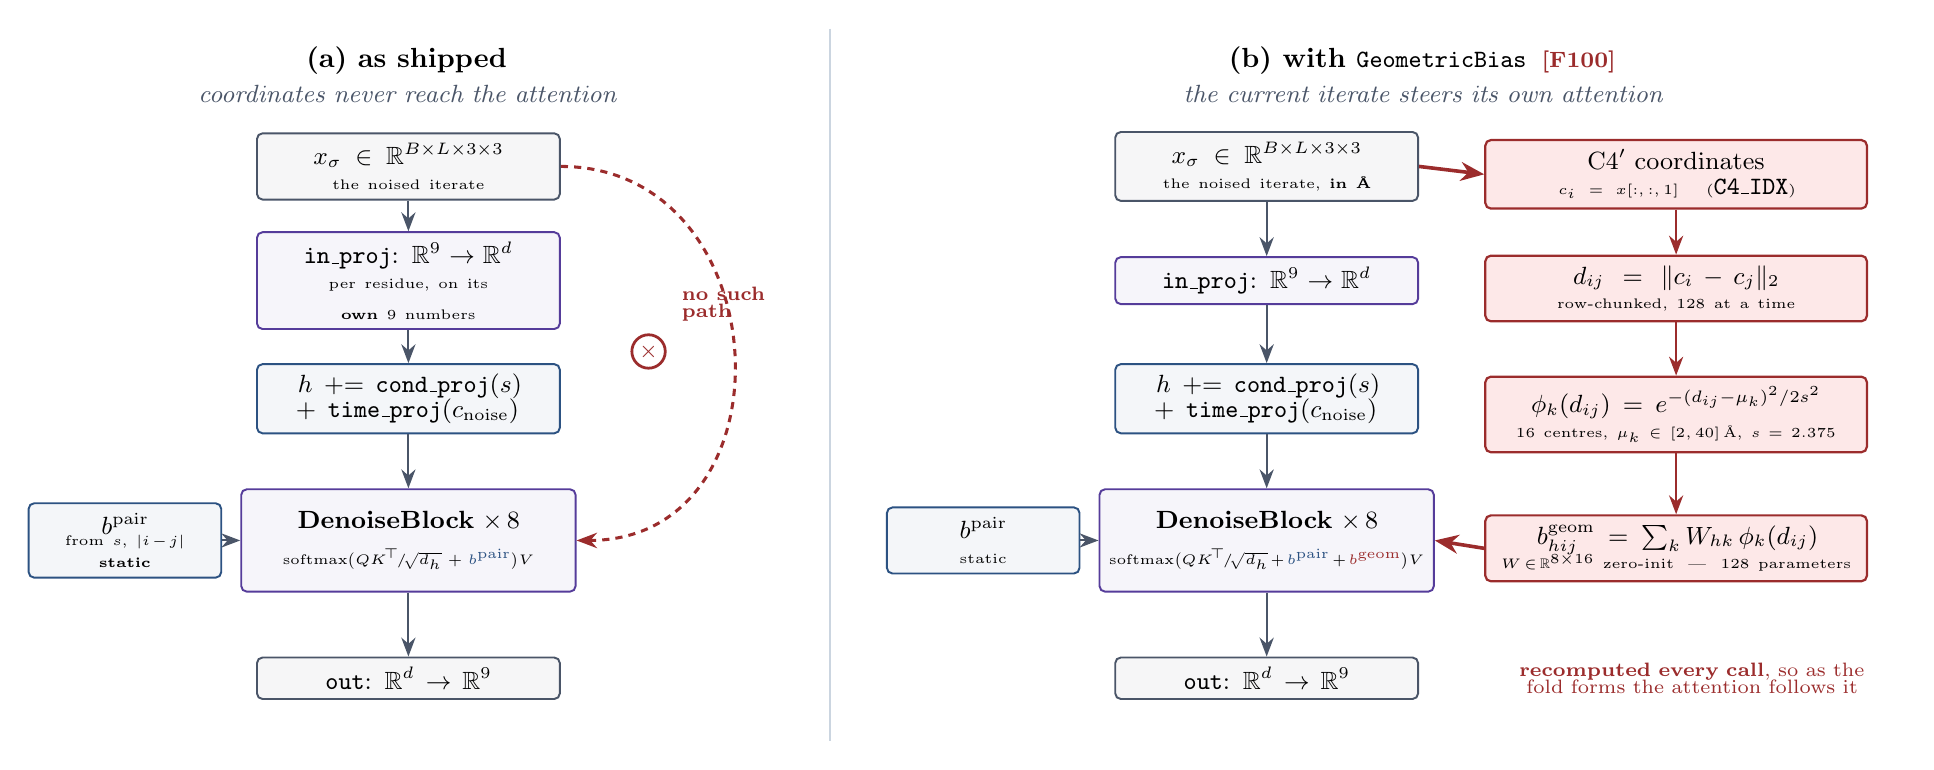
\begin{tikzpicture}[font=\small]
\tikzset{
  dbox/.style={rounded corners=2pt, draw=#1, line width=0.7pt, fill=#1!5,
               align=center, inner sep=3.5pt, font=\small, text width=36mm},
  gbox/.style={rounded corners=2pt, draw=newred, line width=0.8pt,
               fill=newbg, align=center, inner sep=3.5pt, font=\small,
               text width=46mm},
}

% ========================= PANEL (a) =====================================
\begin{scope}[shift={(0,0)}]
  \node[dbox=datagrey]                   at (0,  0   ) (ax)   {$x_\sigma\in\mathbb{R}^{B\times L\times 3\times 3}$\\[-2pt]\tiny the noised iterate};
  \node[dbox=diffpurple]                 at (0, -1.45) (ain)  {\code{in\_proj}: $\mathbb{R}^{9}\!\to\!\mathbb{R}^{d}$\\[-2pt]\tiny per residue, on its \textbf{own} 9 numbers};
  \node[dbox=trunkblue]                  at (0, -2.95) (aadd) {$h \mathrel{+}= \code{cond\_proj}(s)$\\[-2pt]$+\;\code{time\_proj}(c_{\text{noise}})$};
  \node[dbox=diffpurple, text width=40mm, minimum height=13mm]
                                         at (0, -4.75) (ablk) {\textbf{DenoiseBlock} $\times\,8$\\[2pt]\tiny$\softmax\!\big(QK^{\!\top}\!/\!\sqrt{d_h}+\textcolor{trunkblue}{b^{\text{pair}}}\big)V$};
  \node[dbox=trunkblue, text width=22mm] at (-3.6,-4.75) (apair){$b^{\text{pair}}$\\[-2pt]\tiny from $s$, $|i\!-\!j|$\\[-3pt]\tiny\textbf{static}};
  \node[dbox=datagrey]                   at (0, -6.5 ) (aout) {\code{out}: $\mathbb{R}^{d}\!\to\!\mathbb{R}^{9}$};

  \draw[flow] (ax) -- (ain);  \draw[flow] (ain) -- (aadd);
  \draw[flow] (aadd) -- (ablk); \draw[flow] (apair) -- (ablk);
  \draw[flow] (ablk) -- (aout);

  % the path that does not exist
  \draw[line width=1.1pt, draw=newred, dash pattern=on 2.6pt off 2.2pt,
        -{Stealth[length=2.6mm]}]
     (ax.east) to[out=0,in=0,looseness=1.5] (ablk.east);
  \node[draw=newred, fill=white, line width=1pt, circle, inner sep=1.2pt,
        font=\bfseries\footnotesize, text=newred] at (3.05,-2.35) (axx) {$\times$};
  \node[font=\scriptsize\bfseries, text=newred, align=left, anchor=west]
     at (3.35,-1.75) {no such\\[-2pt]path};
\end{scope}

% ========================= PANEL (b) =====================================
\begin{scope}[shift={(10.9,0)}]
  \node[dbox=datagrey]                   at (0,  0   ) (bx)   {$x_\sigma\in\mathbb{R}^{B\times L\times 3\times 3}$\\[-2pt]\tiny the noised iterate, \textbf{in \Ang}};
  \node[dbox=diffpurple]                 at (0, -1.45) (bin)  {\code{in\_proj}: $\mathbb{R}^{9}\!\to\!\mathbb{R}^{d}$};
  \node[dbox=trunkblue]                  at (0, -2.95) (badd) {$h \mathrel{+}= \code{cond\_proj}(s)$\\[-2pt]$+\;\code{time\_proj}(c_{\text{noise}})$};
  \node[dbox=diffpurple, text width=40mm, minimum height=13mm]
                                         at (0, -4.75) (bblk) {\textbf{DenoiseBlock} $\times\,8$\\[2pt]\tiny$\softmax\!\big(QK^{\!\top}\!/\!\sqrt{d_h}+\textcolor{trunkblue}{b^{\text{pair}}}+\textcolor{newred}{b^{\text{geom}}}\big)V$};
  \node[dbox=trunkblue, text width=22mm] at (-3.6,-4.75) (bpair){$b^{\text{pair}}$\\[-2pt]\tiny static};
  \node[dbox=datagrey]                   at (0, -6.5 ) (bout) {\code{out}: $\mathbb{R}^{d}\!\to\!\mathbb{R}^{9}$};

  % --- the new path, in its own column ---
  \node[gbox] at (5.2, -0.1 ) (bc4)  {$\mathrm{C4}'$ coordinates\\[-2pt]\tiny$c_i = x[:,:,1]$ \quad(\code{C4\_IDX})};
  \node[gbox] at (5.2, -1.55) (bd)   {$d_{ij}=\lVert c_i-c_j\rVert_2$\\[-2pt]\tiny row-chunked, $128$ at a time};
  \node[gbox] at (5.2, -3.15) (brbf) {$\phi_k(d_{ij})=e^{-(d_{ij}-\mu_k)^2/2s^2}$\\[-2pt]\tiny $16$ centres, $\mu_k\in[2,40]\,\Ang$, $s=2.375$};
  \node[gbox] at (5.2, -4.85) (bpr)  {$b^{\text{geom}}_{hij}=\sum_k W_{hk}\,\phi_k(d_{ij})$\\[-2pt]\tiny $W\!\in\!\mathbb{R}^{8\times16}$ zero-init \;|\; $128$ parameters};

  \draw[flow] (bx) -- (bin);  \draw[flow] (bin) -- (badd);
  \draw[flow] (badd) -- (bblk); \draw[flow] (bpair) -- (bblk);
  \draw[flow] (bblk) -- (bout);

  \draw[flowthick, draw=newred] (bx.east) -- (bc4.west);
  \draw[flow, draw=newred] (bd)  -- (brbf);
  \draw[flow, draw=newred] (bc4) -- (bd);
  \draw[flow, draw=newred] (brbf)-- (bpr);
  \draw[flowthick, draw=newred] (bpr.west) -- (bblk.east);

  \node[note, text=newred, align=center, text width=52mm] at (5.4,-6.5)
     {\textbf{recomputed every call}, so as the\\[-2pt]
      fold forms the attention follows it};
\end{scope}

% ========================= titles & divider ==============================
\node[font=\bfseries, align=center, text width=72mm] at (0, 1.35)
   {(a) as shipped};
\node[font=\small\itshape, align=center, text width=76mm, text=datagrey] at (0, 0.92)
   {coordinates never reach the attention};
\node[font=\bfseries, align=center, text width=90mm] at (12.9, 1.35)
   {(b) with \code{GeometricBias} \fnd{100}};
\node[font=\small\itshape, align=center, text width=94mm, text=datagrey] at (12.9, 0.92)
   {the current iterate steers its own attention};

\draw[rule1, line width=0.7pt] (5.35,1.75) -- (5.35,-7.3);
\end{tikzpicture}
}
\caption{\textbf{Finding 100.} The decoder had no mechanism by which one
residue's position could influence another's update. Coordinates entered
through a per-residue linear map of that residue's own nine numbers, and
the attention bias was built once from hidden states and relative
\emph{sequence} position. Two residues $6\,\Ang$ apart in space were, to
this attention, exactly as unrelated as two $60\,\Ang$ apart.}
\label{fig:decoder}
\end{figure}

This is the architectural claim of the report, so it is worth stating
carefully. In the shipped decoder,
\begin{equation}
h \leftarrow \code{in\_proj}\big(\mathrm{vec}(x_\sigma)_i\big)
  + \code{cond\_proj}(s_i) + \code{time\_proj}(c_{\text{noise}}),
\qquad
h \leftarrow \mathrm{Block}(h,\; b^{\text{pair}}),
\end{equation}
where $\mathrm{vec}(x_\sigma)_i$ is residue $i$'s own nine coordinates and
$b^{\text{pair}}$ is a function of $s$ and $|i-j|$ only. Neither term
couples residue $i$ to \emph{where residue $j$ currently is}.

This predicts exactly the failure we observe. Bonds come out right,
because relative sequence position suffices for a bond. The fold comes
out wrong, because nothing couples distant residues by proximity. And
feeding the decoder a predicted contact map changed nothing
(finding~93, $+0.0025$ TM against a $0.0023$ noise floor, sign test
$p = 0.50$) --- because a static map is not current geometry: to decide
how to move an atom the model must know where it is \emph{now}.

The fix embeds the pairwise C4$'$ distances of the current iterate in a
16-centre radial basis over $2$--$40\,\Ang$ and projects to a per-head
additive attention bias,
\begin{equation}
b^{\text{geom}}_{hij} = \sum_{k} W_{hk}\,
  \exp\!\left(-\frac{(d_{ij}-\mu_k)^2}{2s^2}\right),
\qquad d_{ij} = \lVert c_i - c_j \rVert_2 ,
\end{equation}
recomputed on every call so the attention follows the structure as it
forms. $W$ is zero-initialised, so a loaded checkpoint's forward pass is
bit-identical until the bias earns its way in. The whole cost is
\textbf{128 parameters}.

Properties pinned by test: zero at initialisation; symmetric; SE(3)
invariant to $2.03\times10^{-6}$, which matters because the loss augments
with random rotations; and --- the property that was absent --- moving
one residue changes the predicted update for \emph{the others}.

\paragraph{Two defects in the fix itself.} The first version was fed
$x_\sigma$, which is $c_{\text{in}}x$ and not \aa ngstr\"oms. At the
median $\sigma$ that divides every distance by 18.7, putting the entire
informative range below the first basis centre and cutting summed
per-channel resolving power from 11.42 to \textbf{0.72}. It would have
trained to nothing while all six tests passed, because all six called the
module directly with \aa ngstr\"oms --- the module was right and its
caller was wrong. The second built its basis in fp32 inside a bf16
autocast region and cost twice the activation memory it needed, which
turned a run that had always fitted into a fatal out-of-memory at
epoch 25 of 40. Both are in the register as 100b and 104b.

% =========================================================================
\section{The pair representation is not constrained to be geometry}
\label{sec:triangle}

\S\ref{sec:decoder} is one half of the global-structure failure. This is
the other, and it is a different gap.

\begin{figure}[H]\centering
\resizebox{\textwidth}{!}{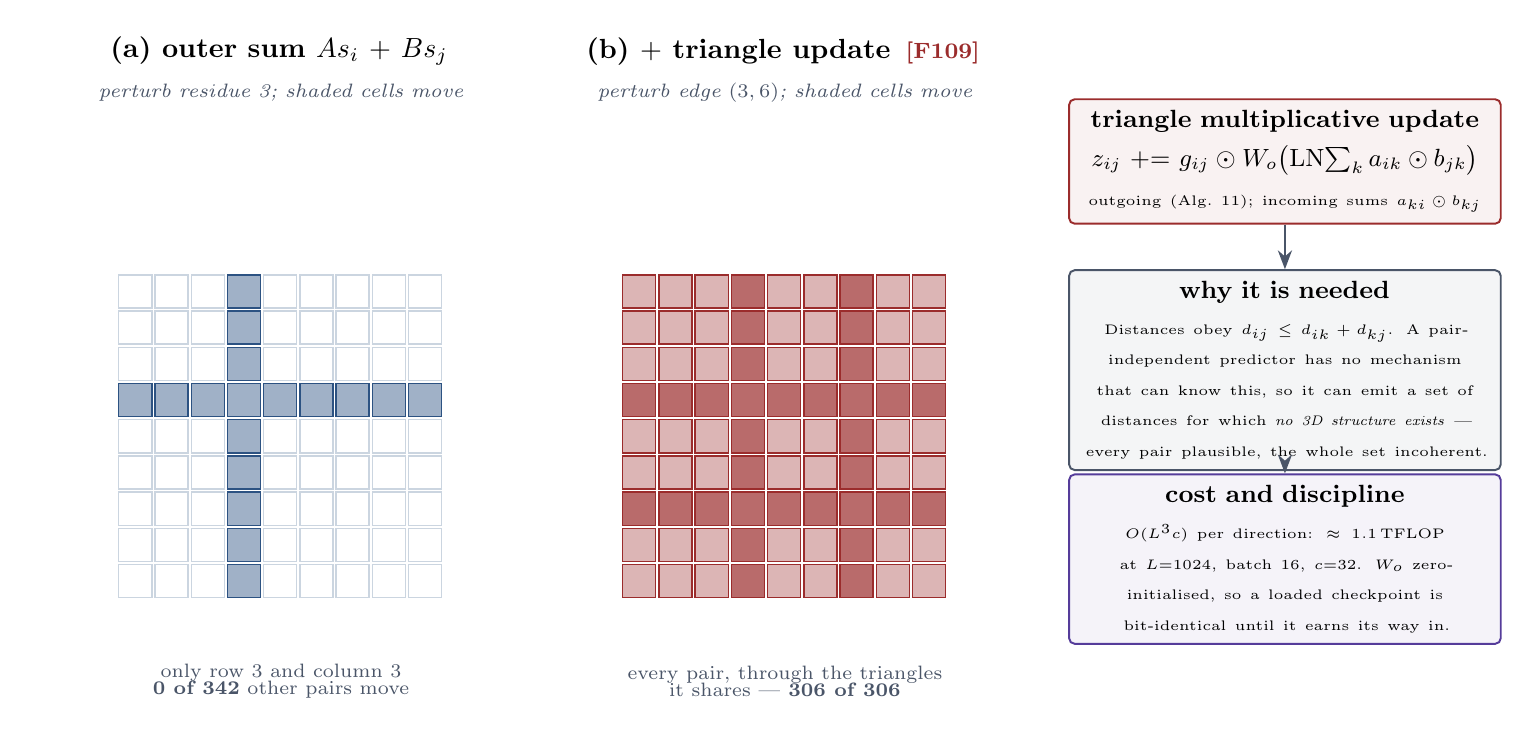
\begin{tikzpicture}[font=\small]
\tikzset{
  cell/.style={draw=#1, line width=0.5pt, minimum size=4.2mm, inner sep=0pt},
  bx/.style={rounded corners=2pt, draw=#1, line width=0.7pt, fill=#1!6,
             align=center, inner sep=4pt, font=\small},
}
\def\N{9}

% ---------------- (a) the outer sum --------------------------------------
\begin{scope}[shift={(0,0)}]
  \node[font=\bfseries, text width=62mm, align=center] at (1.85,3.05)
     {(a) outer sum $A s_i + B s_j$};
  \node[font=\scriptsize\itshape, text=datagrey, text width=58mm, align=center] at (1.85,2.52)
     {perturb residue 3; shaded cells move};
  \foreach \i in {0,...,8}{\foreach \j in {0,...,8}{
     \pgfmathtruncatemacro{\hit}{(\i==3 || \j==3) ? 1 : 0}
     \ifnum\hit=1
       \node[cell=trunkblue, fill=trunkblue!45] at (\i*4.6mm, -\j*4.6mm) {};
     \else
       \node[cell=rule1, fill=white] at (\i*4.6mm, -\j*4.6mm) {};
     \fi}}
  \node[font=\scriptsize, align=center, text=datagrey] at (1.85,-4.95)
     {only row 3 and column 3\\[-2pt]
      \textbf{0 of 342} other pairs move};
\end{scope}

% ---------------- (b) the triangle update --------------------------------
\begin{scope}[shift={(6.4,0)}]
  \node[font=\bfseries, text width=62mm, align=center] at (1.85,3.05)
     {(b) $+$ triangle update \fnd{109}};
  \node[font=\scriptsize\itshape, text=datagrey, text width=58mm, align=center] at (1.85,2.52)
     {perturb edge $(3,6)$; shaded cells move};
  \foreach \i in {0,...,8}{\foreach \j in {0,...,8}{
     \node[cell=newred, fill=newred!35] at (\i*4.6mm, -\j*4.6mm) {};}}
  \foreach \i in {0,...,8}{
     \node[cell=newred, fill=newred!70] at (\i*4.6mm, -3*4.6mm) {};
     \node[cell=newred, fill=newred!70] at (3*4.6mm, -\i*4.6mm) {};
     \node[cell=newred, fill=newred!70] at (\i*4.6mm, -6*4.6mm) {};
     \node[cell=newred, fill=newred!70] at (6*4.6mm, -\i*4.6mm) {};}
  \node[font=\scriptsize, align=center, text=datagrey] at (1.85,-4.95)
     {every pair, through the triangles\\[-2pt]
      it shares --- \textbf{306 of 306}};
\end{scope}

% ---------------- the mechanism ------------------------------------------
\begin{scope}[shift={(14.6,0.1)}]
  \node[bx=newred, text width=52mm] at (0,1.55) (eq)
    {\textbf{triangle multiplicative update}\\[3pt]
     $z_{ij} \mathrel{+}= g_{ij}\odot W_o\!\left(
        \mathrm{LN}\!\sum_k a_{ik}\odot b_{jk}\right)$\\[3pt]
     \tiny outgoing (Alg.\ 11); incoming sums $a_{ki}\odot b_{kj}$};
  \node[bx=datagrey, text width=52mm] at (0,-1.1) (why)
    {\textbf{why it is needed}\\[2pt]
     \tiny Distances obey $d_{ij} \le d_{ik} + d_{kj}$. A pair-independent
     predictor has no mechanism that can know this, so it can emit a set of
     distances for which \emph{no 3D structure exists} --- every pair
     plausible, the whole set incoherent.};
  \node[bx=diffpurple, text width=52mm] at (0,-3.5) (cost)
    {\textbf{cost and discipline}\\[2pt]
     \tiny $O(L^3c)$ per direction: $\approx1.1$\,TFLOP at $L{=}1024$,
     batch 16, $c{=}32$. $W_o$ zero-initialised, so a loaded checkpoint is
     bit-identical until it earns its way in.};
  \draw[flow] (eq) -- (why); \draw[flow] (why) -- (cost);
\end{scope}
\end{tikzpicture}
}
\caption{\textbf{Finding 109.} \code{DiffusionPairFeatures} is an outer
sum, so $z_{ij}$ is a function of its two endpoints and of nothing else.
Measured, not inferred: perturb one residue's hidden state and
\textbf{0 of 342} pairs that exclude it move. With the triangle update,
\textbf{306 of 306} do.}
\label{fig:triangle}
\end{figure}

The pair representation the decoder reads is
\begin{equation}
z_{ij} = \mathrm{LN}\!\big(A s_i + B s_j + R_{\mathrm{clamp}(j-i)}
         + C\,\mathrm{coev}_{ij}\big),
\end{equation}
an outer \emph{sum}. Its own docstring is candid about the limitation ---
``it cannot represent interactions between the two endpoints that are not
additive, and the attention layers above it exist to supply those'' ---
but finding 92 measured those attention layers at chance against the
contact map, so the non-additive part is not in fact being supplied.

We measured the consequence directly. Perturbing residue 3's hidden state
moves all 48 pair entries that involve residue 3, and \textbf{0 of the
342} that do not. That is what an outer sum must give, and it is the
precise sense in which the pair track cannot be geometry: distances obey
$d_{ij} \le d_{ik} + d_{kj}$, and a predictor whose pairs are mutually
independent has no mechanism that can know it. Such a model can emit a
set of pairwise distances \emph{for which no three-dimensional structure
exists at all} --- every pair locally plausible, the whole set globally
incoherent.

Seen from outside, that is lDDT $0.269$ beside TM $0.094$.

The triangle multiplicative update is the standard remedy and the one
ingredient of the AlphaFold-class pair stack this model never had. With
$a, b$ gated projections to $c$ channels,
\begin{equation}
z_{ij} \mathrel{+}= g_{ij} \odot W_o\!\left(
  \mathrm{LN}\sum_k a_{ik} \odot b_{jk}\right)
\quad\text{(outgoing)},\qquad
\sum_k a_{ki} \odot b_{kj} \quad\text{(incoming)} .
\end{equation}
Two rounds at $c = 32$ against $d_{\text{pair}} = 160$: the triangle term
is a \emph{constraint} on the pair track, not a replacement for it. The
cost is $O(L^3 c)$ per direction, about $1.1$\,TFLOP at $L = 1024$ and
batch 16, and $W_o$ is zero-initialised so a loaded checkpoint is
bit-identical until the update earns its way in.

\paragraph{And the pair feature is the wrong shape for base pairing.}
The outer sum has a second defect, separate from the triangle one and
sharper. ``$i$ pairs with $j$'' is a statement about the two
\emph{together}; a sum of per-endpoint terms cannot express it. Fitted to
a toy A--U/C--G rule ($\mathrm{type}_i + \mathrm{type}_j = 3$):

\begin{center}\small
\begin{tabular}{lr}
\toprule
shape & accuracy \\
\midrule
outer sum $A h_i + B h_j$ & \textbf{0.681} \\
always-zero baseline & \textbf{0.743} \\
bilinear $\langle U h_i, V h_j\rangle$ & \textbf{1.000} \\
\bottomrule
\end{tabular}
\end{center}

The sum does not merely do worse --- it cannot beat predicting ``no
pair'' everywhere, while a bilinear form fits the rule exactly. This is
one toy problem rather than a corpus measurement, and that is the weight
it should carry; but base pairing \emph{is} complementarity, and the
pair track is additive in its endpoints.

\code{ContactBias} supplies the bilinear form to the trunk's two
\code{full} blocks through the \code{pair\_bias\_fn} recycling hook they
already have --- computed from loop $k$, biasing loop $k{+}1$, so it
needs no extra pass. 50,689 parameters at rank 32, zero-gated.

\paragraph{Everything in this section is implemented and switched off.}
\code{triangle\_layers} defaults to $0$, as do \code{bidirectional\_gdn}
and \code{contact\_bias}. Five unmeasured changes landing together would
confound all five, so each is a separate queued arm from the same
stage-4 initialisation at the baseline's settings, and
\S\ref{sec:results} reports no outcome for any of them.

% =========================================================================
\section{Heads, losses and curriculum}

\begin{table}[H]\centering\small
\begin{tabular}{clllr}
\toprule
\# & head & predicts & loss & weight \\
\midrule
1  & contact   & heavy-atom contact $<8\,\Ang$, $|i-j|\ge4$ & BCE, quality-weighted & 1.0 \\
2  & distance  & C4$'$--C4$'$, 40 bins & cross-entropy & 0.5 \\
3  & structure & backbone $(\mathrm{P},\mathrm{C4}',\mathrm{N})$ & EDM $+$ violation & 1.0 \\
4  & secondary & dot-bracket, 8 symbols & cross-entropy & 0.5 \\
5  & reactivity& SHAPE and DMS & smooth-$L_1$ & 1.0 \\
6  & Mg$^{2+}$ & ion within $3\,\Ang$ & BCE, clamped pos-weight & 0.3 \\
7  & rigidity  & $z$-scored B-factor, X-ray only & smooth-$L_1$ & 0.3 \\
8  & disorder  & unobserved residue & \textcolor{newred}{none} & --- \\
9  & geometry  & Leontis--Westhof class, 13 & cross-entropy & 0.5 \\
10 & motif     & hairpin / internal / neither & cross-entropy & 0.3 \\
11 & torsion   & $\eta,\theta,\tilde\chi$ as $(\sin,\cos)$ & unit-circle $+$ norm & 0.3 \\
\midrule
-- & base identity & 4 classes & cross-entropy & 0.2 \\
-- & fluctuation   & ensemble amplitude & smooth-$L_1$ & 0.1 \\
-- & fitness       & variant fitness & MSE & 0.3 \\
-- & splice, ensemble state & --- & \textcolor{newred}{none} & --- \\
\bottomrule
\end{tabular}
\caption{The head inventory. Three outputs are emitted and never trained:
disorder needs \texttt{entity\_poly\_seq} in the corpus, splice needs a
corpus that has not been acquired, and no observable distinguishes the
$K$ ensemble states. They are recorded as untrained rather than quietly
reported.}
\end{table}

\paragraph{Torsions.} Head 11 predicts the Duarte--Pyle pseudotorsions
$\eta_i = \angle(\mathrm{C4}'_{i-1},\mathrm{P}_i,\mathrm{C4}'_i,\mathrm{P}_{i+1})$,
$\theta_i = \angle(\mathrm{P}_i,\mathrm{C4}'_i,\mathrm{P}_{i+1},\mathrm{C4}'_{i+1})$
and
$\tilde\chi_i = \angle(\mathrm{P}_i,\mathrm{C4}'_i,\mathrm{N}_i,\mathrm{P}_{i+1})$
as unnormalised $(\sin,\cos)$ pairs, with loss
$\lVert u - t\rVert^2 = 2 - 2\cos\Delta$ on the normalised vector plus
$0.02\,\big||p| - 1\big|$ on its magnitude. They are computed from batch
coordinates on the fly, never stored.

\paragraph{Distance bins.} 40 bins: eight uniform of $0.875\,\Ang$ over
$3$--$10\,\Ang$, then 32 equal-frequency edges to $100.78\,\Ang$ with the
last open-ended. Uniform binning over the whole range had put the
majority class at a level the head could reach by constant prediction,
which is finding 75.

\begin{figure}[H]\centering
\resizebox{0.96\textwidth}{!}{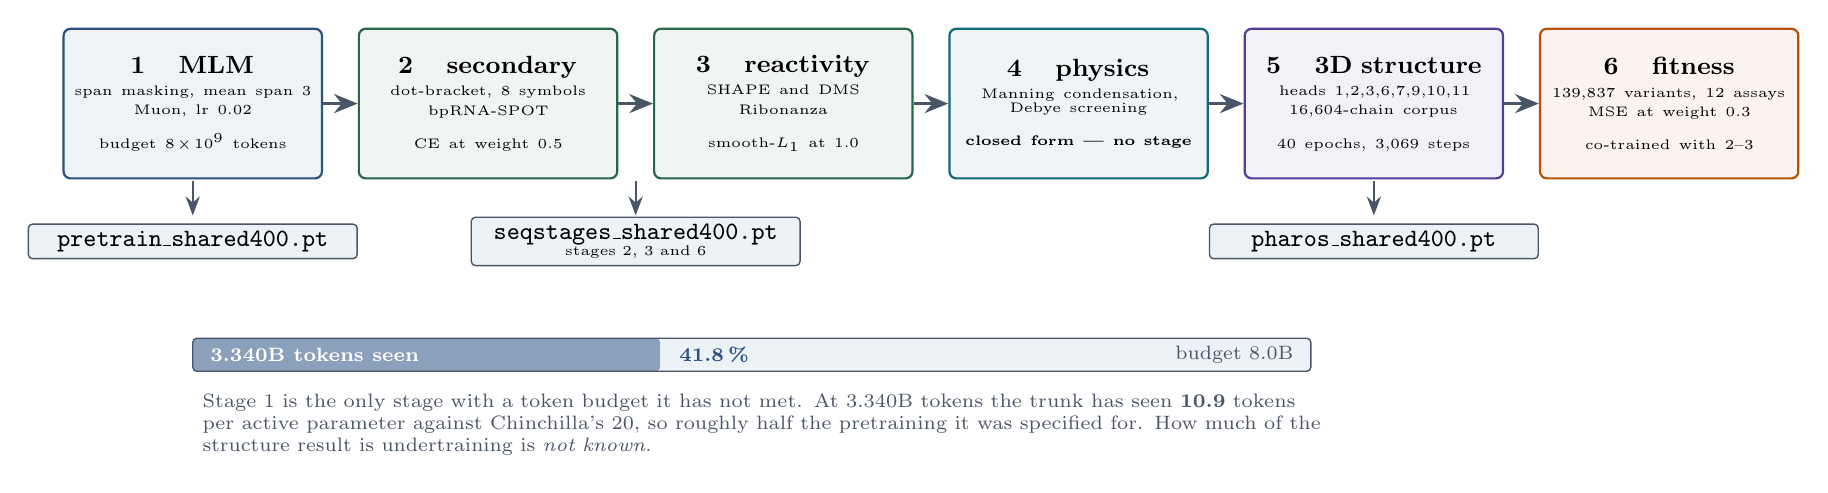
\begin{tikzpicture}[font=\small]
\tikzset{
  sg/.style={rounded corners=2.5pt, draw=#1, line width=0.8pt, fill=#1!7,
             align=center, inner sep=4pt, font=\small, text width=30mm,
             minimum height=19mm},
  ck/.style={rounded corners=1.5pt, draw=datagrey, line width=0.5pt,
             fill=databg, align=center, inner sep=2.5pt, font=\tiny,
             text width=40mm},
}
\def\dx{3.75}

\node[sg=trunkblue]  at (0*\dx,0) (s1)
  {\textbf{1 \;\; MLM}\\[2pt]\tiny span masking, mean span 3\\[1pt]
   \tiny Muon, lr 0.02\\[1pt]\tiny budget $8\!\times\!10^{9}$ tokens};
\node[sg=headgreen]  at (1*\dx,0) (s2)
  {\textbf{2 \;\; secondary}\\[2pt]\tiny dot-bracket, 8 symbols\\[1pt]
   \tiny bpRNA-SPOT\\[1pt]\tiny CE at weight 0.5};
\node[sg=headgreen]  at (2*\dx,0) (s3)
  {\textbf{3 \;\; reactivity}\\[2pt]\tiny SHAPE and DMS\\[1pt]
   \tiny Ribonanza\\[1pt]\tiny smooth-$L_1$ at 1.0};
\node[sg=physteal]   at (3*\dx,0) (s4)
  {\textbf{4 \;\; physics}\\[2pt]\tiny Manning condensation,\\[-1pt]
   \tiny Debye screening\\[1pt]\tiny\textbf{closed form --- no stage}};
\node[sg=diffpurple] at (4*\dx,0) (s5)
  {\textbf{5 \;\; 3D structure}\\[2pt]\tiny heads 1,2,3,6,7,9,10,11\\[1pt]
   \tiny 16{,}604-chain corpus\\[1pt]\tiny 40 epochs, 3{,}069 steps};
\node[sg=moeorange]  at (5*\dx,0) (s6)
  {\textbf{6 \;\; fitness}\\[2pt]\tiny 139{,}837 variants, 12 assays\\[1pt]
   \tiny MSE at weight 0.3\\[1pt]\tiny co-trained with 2--3};

\foreach \a/\b in {s1/s2, s2/s3, s3/s4, s4/s5, s5/s6}{
  \draw[flowthick] (\a) -- (\b);}

\node[ck] at (0*\dx,-1.75) {\code{pretrain\_shared400.pt}};
\node[ck] at (1.5*\dx,-1.75) {\code{seqstages\_shared400.pt}\\stages 2, 3 and 6};
\node[ck] at (4*\dx,-1.75) {\code{pharos\_shared400.pt}};
\foreach \x in {0, 1.5, 4}{
  \draw[flow, draw=datagrey] (\x*\dx,-0.98) -- (\x*\dx,-1.42);}

% stage-1 progress bar
\begin{scope}[shift={(0,-3.4)}]
  \def\W{14.2}
  \fill[databg, rounded corners=1.5pt] (0,0) rectangle (\W,0.42);
  \fill[trunkblue!55, rounded corners=1.5pt] (0,0) rectangle (0.418*\W,0.42);
  \draw[datagrey, line width=0.5pt, rounded corners=1.5pt] (0,0) rectangle (\W,0.42);
  \node[font=\scriptsize, text=white, anchor=west] at (0.1,0.21)
     {\textbf{3.340B tokens seen}};
  \node[font=\scriptsize, text=datagrey, anchor=east] at (\W-0.1,0.21)
     {budget $8.0$B};
  \node[font=\scriptsize\bfseries, text=trunkblue, anchor=west] at (0.418*\W+0.12,0.21)
     {41.8\,\%};
  \node[note, anchor=north west, text width=\W cm] at (0,-0.16)
     {\scriptsize Stage 1 is the only stage with a token budget it has not
      met. At 3.340B tokens the trunk has seen \textbf{10.9} tokens per
      active parameter against Chinchilla's 20, so roughly half the
      pretraining it was specified for. How much of the structure result
      is undertraining is \emph{not known}.};
\end{scope}
\end{tikzpicture}
}
\caption{\textbf{The six-stage curriculum.} Each stage initialises from
the previous one's checkpoint, and the driver refuses to start a stage
from random weights.}
\label{fig:curriculum}
\end{figure}

% =========================================================================
\section{Results}
\label{sec:results}

\subsection{What the heads learn}

At the end of a 40-epoch stage-5 run (3{,}069 optimiser steps,
16{,}384-token budget) on the held-out test split:

\begin{table}[H]\centering\small
\begin{tabular}{lrr}
\toprule
metric & value & reference \\
\midrule
contact average precision & \textbf{0.8901} & base rate \textbf{0.4541} \fnd{107} \\
Mg$^{2+}$ average precision & 0.4167 & base rate 0.0254 ($16.4\times$) \\
Leontis--Westhof accuracy & 0.8972 & majority 0.8532 \\
motif accuracy & 0.7494 & majority 0.6925 \\
$\eta$ MAE & $23.29^\circ$ & circular baseline $24.59^\circ$ \\
$\theta$ MAE & $26.86^\circ$ & circular baseline $29.05^\circ$ \\
$\tilde\chi$ MAE & $16.21^\circ$ & circular baseline $17.74^\circ$ \\
structure MSE & 24.59 & --- \\
P--P bond violation & 0.1934 & target $6.01\,\Ang$ \\
\bottomrule
\end{tabular}
\end{table}

Torsions beat their circular baselines by $1.3$--$2.2^\circ$, which is
real but small. Ion sites are $16\times$ better than chance.

\paragraph{The contact number needs a caveat, and it is a large one.}
That average precision is computed on pairs from \code{sample\_pairs},
which takes \emph{every} positive plus at most 512 sampled negatives, so
the set it scores is \textbf{45.4\,\% positive}. The task --- every pair
with $|i-j| \ge 4$ --- is \textbf{9.6\,\% positive} on this corpus, which
we measured directly over 200 test chains. Average precision moves with
the base rate, so $0.8901$ at a $0.4541$ base is not comparable to a
published contact-prediction figure, and the honest normalised form is
the lift the code also reports: $1.96\times$ base. The full-pair-set
metric is implemented and has not yet been run, because it needs a GPU
(finding 107).

This matters beyond bookkeeping: $0.890$ is the number
\S\ref{sec:results} and finding 92 use to argue that contacts are
predicted well while the fold is not, and that argument is what sent the
search into the decoder. It may survive --- see below --- but it has not
been tested on the task it claims.

\paragraph{One hypothesis, tested and refuted.} The pair feature is an
outer sum $A s_i + B s_j$, which can score well by knowing \emph{which}
residues are paired without knowing \emph{with whom} --- and that would
have explained AP $0.89$ beside TM $0.09$ neatly. It does not. A
partner-blind oracle handed the \emph{true} degree of every residue
reaches only AP $0.3005$ on the real pair set, against a $0.0961$ base
and $0.1209$ for sequence separation alone. The head sits far above that,
so it does carry genuine pairing-partner information.

\subsection{What the model does not do}

\begin{table}[H]\centering\small
\begin{tabular}{lrrrr}
\toprule
& run 1 & run 2 & run 3 & field median \\
\midrule
mean TM-score & 0.0890 & 0.0913 & \textbf{0.0936} & \textbf{0.3013} \\
mean lDDT     & 0.2550 & 0.2765 & 0.2690 & --- \\
targets above field median & 0/17 & 0/17 & 0/17 & --- \\
targets above TM 0.45 & 0/17 & 0/17 & 0/17 & --- \\
\bottomrule
\end{tabular}
\caption{17 RNA-Puzzles targets, scored against all submitted competitor
models. Three runs at identical settings span $0.0046$ against a
$0.0023$ initialisation-noise floor measured between two of them.
Nothing has moved.}
\end{table}

The mean percentile against the field is 99.7\,\%: last or near-last on
15 of 17 targets.

\paragraph{The diagnostic.} lDDT $0.269$ beside TM $0.094$ is the whole
story. lDDT is a local measure --- it asks whether each residue's
neighbourhood is right --- and TM is a global one. A model that scored
badly on both would be producing noise. A model that scores
\emph{moderately} on the local measure and at floor on the global one is
producing locally-valid RNA backbone in the wrong global arrangement.
That is consistent with every other number here: bonds within tolerance,
contacts at AP $0.890$, torsions beating their baselines, and a fold that
is wrong.

\paragraph{What has been ruled out.} Chain breaks: 99.09\,\% of
2{,}227{,}344 P--P pairs lie inside tolerance. Stage-1 representation
quality: sequence explains $0.92\%$ of P--P distance variance, so the
bond is a geometric constant and not something the language model must
supply. Decoder access to contacts: supplying a predicted contact map
moved TM by $+0.0025$ against a $0.0023$ noise floor, 9 wins in 17, sign
test $p = 0.50$ (finding 93, reverted).

What that leaves is the decoder's ability to \emph{use} geometry, which
is \S\ref{sec:decoder} and finding 100. At the time of writing that A/B
has completed 25 of 40 epochs and \textbf{no claim is made about its
outcome}. At matched epochs the two arms are indistinguishable on
structure loss; the bias itself is demonstrably learning, with per-head
attention offsets that are positive at $6$--$12\,\Ang$ and negative at
$23$--$40\,\Ang$, which is the correct sign structure.

% =========================================================================
\section{The defect register as method}
\label{sec:register}

The repository carries \code{research/architecture/FINDINGS.md}, at
present 104 numbered entries. It is not a changelog. Its recurring class
is narrow and worth naming:

\begin{quote}
\emph{a component that exists, is measured, and whose output is never
checked for basic validity.}
\end{quote}

Representative entries:

\begin{itemize}
\item \textbf{85} --- $P_{\text{mean}}$ carried over from a paper that
  used $\sigma_d = 0.5$, leaving the denoiser responsible for $0.035\%$
  of its task at the median training draw.
\item \textbf{90} --- the inference sampler passed \code{pair=None},
  withholding relative position from the decoder at sampling time only.
  P--P went from $16$--$19\,\Ang$ to $5.53$--$6.43\,\Ang$ against a true
  $5.95$.
\item \textbf{102} --- the active parameter count costed a token at
  $\texttt{max\_k}/4 = 128$ experts while an audit file in the same
  repository recorded a measured width of 15.28. Both numbers were on
  disk; nothing compared them.
\item \textbf{104} --- the training loop skipped out-of-memory batches
  and the validation ten lines below it did not, so a batch that costs
  one gradient in training killed a 40-epoch run at epoch 25.
\end{itemize}

Three disciplines follow from this, and they are the reason the negative
results in \S\ref{sec:results} can be relied on.

\paragraph{Every new pathway is zero-initialised.} \code{bias\_scale},
\code{site\_scale}, \code{coev\_proj}, \code{recycle\_proj} and
\code{GeometricBias.proj} all start at exactly zero, so adding a feature
cannot regress a working checkpoint and the feature has to earn its
contribution.

\paragraph{Every metric is reported against its floor.} Accuracy against
the majority class, average precision against the base rate, angular MAE
against the circular mean, correlation pooled over the split rather than
averaged per batch. Finding 75 was a head that looked like it was
learning because its floor had never been computed.

\paragraph{Refutations are recorded as prominently as confirmations.}
The register contains a withdrawn finding (76, where we measured our own
interference and blamed the code), a refuted experiment (93), a
corrected claim (a $+0.2761$ distance lift computed against a floor
sampled over different batches), and a section titled \emph{Checked and
not defects}. Twenty-two of a monitoring script's first twenty-three
warnings were false positives, and fixing the script was treated as
equal in value to fixing the model.

% =========================================================================
\section{Limitations, and what we think is wrong}

\begin{enumerate}
\item \textbf{The fold is wrong and two candidate fixes are
  unmeasured.} Finding 100 (the decoder could not see current geometry)
  and finding 109 (the pair track is not constrained to be
  three-dimensionally embeddable) each have a mechanism that explains the
  observations and an implementation whose effect is demonstrable on
  synthetic input. Neither has been A/B'd. That is all that can honestly
  be said.

\item \textbf{Two thirds of the trunk cannot see to its right.}
  \texttt{gdn} is strictly causal --- scrambling the right half of the
  input moves the left half of its output by exactly zero. \pharos{} is
  an encoder and nothing in the task asks for a causal mask. We record
  this as declared rather than as a defect, because contact AP of $0.890$
  shows the information does arrive, by two routes that do not need
  \texttt{gdn}: the pair features are an outer sum that sees both
  endpoints, and three recycled passes carry right-context back
  (finding 103).

\item \textbf{The trunk's global attention does not attend to contacts
  --- and was never asked to.} The two \code{full} blocks score AUROC
  $0.44$--$0.52$ against the contact map. On reread that is the expected
  outcome rather than an anomaly: the contact head reads $h_i$ and $h_j$
  directly through the pair track, so it needs nothing from attention;
  the only pair signal those blocks receive is the electrostatic bias,
  measured at $2.6\times10^{-4}$ of a logit; and they are 2 blocks of 18.
  Nothing in the architecture asks attention to encode contacts.
  \code{ContactBias} is the missing mechanism, built and queued
  (finding 92, open).

\item \textbf{The coevolution feature is below its own noise floor for
  most of the corpus.} Chain-weighted, $67.2\,\%$ of family-assigned
  chains sit behind an alignment with Henikoff $N_{\text{eff}} < 50$ and
  the median family reads $4.0$, against a stated MI noise floor of 8
  sequences. A union cache --- full alignment where one exists, seed
  otherwise --- lifts the fraction at $N_{\text{eff}} \ge 50$ from
  $31.9\,\%$ to $58.5\,\%$, with 5S~rRNA (2,235 chains) going
  $12.2 \to 433.5$. Built, measured, queued; $11.3\,\%$ of chains stay
  under $N_{\text{eff}}\,10$ because tRNA and the large rRNAs have no
  full alignment at all (findings 110 and 112).

\item \textbf{Three heads are emitted and untrained}, and one declared
  router feature is read by the model and written by no caller
  (finding 68, open).

\item \textbf{Stage 1 is at 41.8\% of its token budget.} At 3.340B of
  8B tokens the trunk has seen 10.9 tokens per active parameter, about
  half Chinchilla-optimal. Some of the gap is undertraining and we do not
  know how much.

\item \textbf{The fitness head barely transfers.} Validation Spearman
  $+0.604$ over 12 assays of seen constructs against $+0.085$ on a
  held-out aptamer family (finding 97, open).
\end{enumerate}

\paragraph{The honest summary.} \pharos{} is a working multi-task RNA
model with a non-functioning structure decoder. The discriminative heads
do what they were built to do. The generative head does not.

We think we know why, and the account is specific: the decoder could not
see where the atoms were (100), the pair track is not constrained to be
three-dimensionally embeddable (109), it is additive where base pairing
is multiplicative (92), two thirds of the trunk cannot see to its right
(103), and the coevolution channel is below its own noise floor for two
thirds of the corpus (112). Each has an implementation whose effect is
demonstrable on synthetic input and \textbf{none has been measured
against the baseline}. Until they are, this section is a set of
hypotheses with code attached, and the only number that describes the
model is TM $0.094$.

\end{document}
